\documentclass[twoside]{book}

% Packages required by doxygen
\usepackage{calc}
\usepackage{doxygen}
\usepackage{graphicx}
\usepackage[utf8]{inputenc}
\usepackage{makeidx}
\usepackage{multicol}
\usepackage{multirow}
\usepackage{textcomp}
\usepackage[table]{xcolor}

% Font selection
\usepackage[T1]{fontenc}
\usepackage{mathptmx}
\usepackage[scaled=.90]{helvet}
\usepackage{courier}
\usepackage{amssymb}
\usepackage{sectsty}
\renewcommand{\familydefault}{\sfdefault}
\allsectionsfont{%
  \fontseries{bc}\selectfont%
  \color{darkgray}%
}
\renewcommand{\DoxyLabelFont}{%
  \fontseries{bc}\selectfont%
  \color{darkgray}%
}

% Page & text layout
\usepackage{geometry}
\geometry{%
  a4paper,%
  top=2.5cm,%
  bottom=2.5cm,%
  left=2.5cm,%
  right=2.5cm%
}
\tolerance=750
\hfuzz=15pt
\hbadness=750
\setlength{\emergencystretch}{15pt}
\setlength{\parindent}{0cm}
\setlength{\parskip}{0.2cm}
\makeatletter
\renewcommand{\paragraph}{%
  \@startsection{paragraph}{4}{0ex}{-1.0ex}{1.0ex}{%
    \normalfont\normalsize\bfseries\SS@parafont%
  }%
}
\renewcommand{\subparagraph}{%
  \@startsection{subparagraph}{5}{0ex}{-1.0ex}{1.0ex}{%
    \normalfont\normalsize\bfseries\SS@subparafont%
  }%
}
\makeatother

% Headers & footers
\usepackage{fancyhdr}
\pagestyle{fancyplain}
\fancyhead[LE]{\fancyplain{}{\bfseries\thepage}}
\fancyhead[CE]{\fancyplain{}{}}
\fancyhead[RE]{\fancyplain{}{\bfseries\leftmark}}
\fancyhead[LO]{\fancyplain{}{\bfseries\rightmark}}
\fancyhead[CO]{\fancyplain{}{}}
\fancyhead[RO]{\fancyplain{}{\bfseries\thepage}}
\fancyfoot[LE]{\fancyplain{}{}}
\fancyfoot[CE]{\fancyplain{}{}}
\fancyfoot[RE]{\fancyplain{}{\bfseries\scriptsize Generated on Mon Jul 8 2013 13:06:30 for ggPlayer by Doxygen }}
\fancyfoot[LO]{\fancyplain{}{\bfseries\scriptsize Generated on Mon Jul 8 2013 13:06:30 for ggPlayer by Doxygen }}
\fancyfoot[CO]{\fancyplain{}{}}
\fancyfoot[RO]{\fancyplain{}{}}
\renewcommand{\footrulewidth}{0.4pt}
\renewcommand{\chaptermark}[1]{%
  \markboth{#1}{}%
}
\renewcommand{\sectionmark}[1]{%
  \markright{\thesection\ #1}%
}

% Indices & bibliography
\usepackage{natbib}
\usepackage[titles]{tocloft}
\setcounter{tocdepth}{3}
\setcounter{secnumdepth}{5}
\makeindex

% Hyperlinks (required, but should be loaded last)
\usepackage{ifpdf}
\ifpdf
  \usepackage[pdftex,pagebackref=true]{hyperref}
\else
  \usepackage[ps2pdf,pagebackref=true]{hyperref}
\fi
\hypersetup{%
  colorlinks=true,%
  linkcolor=blue,%
  citecolor=blue,%
  unicode%
}

% Custom commands
\newcommand{\clearemptydoublepage}{%
  \newpage{\pagestyle{empty}\cleardoublepage}%
}


%===== C O N T E N T S =====

\begin{document}

% Titlepage & ToC
\hypersetup{pageanchor=false}
\pagenumbering{roman}
\begin{titlepage}
\vspace*{7cm}
\begin{center}%
{\Large gg\-Player \\[1ex]\large 0.\-0 }\\
\vspace*{1cm}
{\large Generated by Doxygen 1.8.4}\\
\vspace*{0.5cm}
{\small Mon Jul 8 2013 13:06:30}\\
\end{center}
\end{titlepage}
\clearemptydoublepage
\tableofcontents
\clearemptydoublepage
\pagenumbering{arabic}
\hypersetup{pageanchor=true}

%--- Begin generated contents ---
\chapter{R\-E\-A\-D\-M\-E}
\label{md_ggplayer_README}
\hypertarget{md_ggplayer_README}{}
\input{md_ggplayer__r_e_a_d_m_e}
\chapter{R\-E\-A\-D\-M\-E}
\label{md_README}
\hypertarget{md_README}{}
\input{md__r_e_a_d_m_e}
\chapter{Namespace Index}
\section{Packages}
Here are the packages with brief descriptions (if available)\-:\begin{DoxyCompactList}
\item\contentsline{section}{\hyperlink{namespace____main____}{\-\_\-\-\_\-main\-\_\-\-\_\-} }{\pageref{namespace____main____}}{}
\item\contentsline{section}{\hyperlink{namespaceboardgame}{boardgame} \\*Package containing the common classes for the gg\-\_\-architecture }{\pageref{namespaceboardgame}}{}
\item\contentsline{section}{\hyperlink{namespacegg__arch}{gg\-\_\-arch} }{\pageref{namespacegg__arch}}{}
\item\contentsline{section}{\hyperlink{namespacegg__arch_1_1boardgame}{gg\-\_\-arch.\-boardgame} }{\pageref{namespacegg__arch_1_1boardgame}}{}
\item\contentsline{section}{\hyperlink{namespacegg__arch_1_1chess}{gg\-\_\-arch.\-chess} }{\pageref{namespacegg__arch_1_1chess}}{}
\item\contentsline{section}{\hyperlink{namespacegg__arch_1_1gamecell}{gg\-\_\-arch.\-gamecell} }{\pageref{namespacegg__arch_1_1gamecell}}{}
\item\contentsline{section}{\hyperlink{namespacegg__arch_1_1gamepiece}{gg\-\_\-arch.\-gamepiece} }{\pageref{namespacegg__arch_1_1gamepiece}}{}
\item\contentsline{section}{\hyperlink{namespacegg_player}{gg\-Player} }{\pageref{namespacegg_player}}{}
\item\contentsline{section}{\hyperlink{namespaceoutput}{output} }{\pageref{namespaceoutput}}{}
\end{DoxyCompactList}

\chapter{Hierarchical Index}
\section{Class Hierarchy}
This inheritance list is sorted roughly, but not completely, alphabetically\-:\begin{DoxyCompactList}
\item object\begin{DoxyCompactList}
\item \contentsline{section}{gg\-\_\-arch.\-boardgame.\-Boardgame}{\pageref{classgg__arch_1_1boardgame_1_1_boardgame}}{}
\item \contentsline{section}{gg\-\_\-arch.\-gamecell.\-game\-Cell}{\pageref{classgg__arch_1_1gamecell_1_1game_cell}}{}
\item \contentsline{section}{gg\-\_\-arch.\-gamepiece.\-Gamepiece}{\pageref{classgg__arch_1_1gamepiece_1_1_gamepiece}}{}
\end{DoxyCompactList}
\item Boardgame\begin{DoxyCompactList}
\item \contentsline{section}{gg\-\_\-arch.\-chess.\-Chess}{\pageref{classgg__arch_1_1chess_1_1_chess}}{}
\end{DoxyCompactList}
\item G\-W\-T\-Canvas\begin{DoxyCompactList}
\item \contentsline{section}{gg\-Player.\-Game\-Canvas}{\pageref{classgg_player_1_1_game_canvas}}{}
\end{DoxyCompactList}
\end{DoxyCompactList}

\chapter{Class Index}
\section{Class List}
Here are the classes, structs, unions and interfaces with brief descriptions\-:\begin{DoxyCompactList}
\item\contentsline{section}{\hyperlink{classgg__arch_1_1boardgame_1_1_boardgame}{gg\-\_\-arch.\-boardgame.\-Boardgame} \\*Copyright 2013 Hans Rinderknecht }{\pageref{classgg__arch_1_1boardgame_1_1_boardgame}}{}
\item\contentsline{section}{\hyperlink{classgg__arch_1_1chess_1_1_chess}{gg\-\_\-arch.\-chess.\-Chess} }{\pageref{classgg__arch_1_1chess_1_1_chess}}{}
\item\contentsline{section}{\hyperlink{classgg_player_1_1_game_canvas}{gg\-Player.\-Game\-Canvas} }{\pageref{classgg_player_1_1_game_canvas}}{}
\item\contentsline{section}{\hyperlink{classgg__arch_1_1gamecell_1_1game_cell}{gg\-\_\-arch.\-gamecell.\-game\-Cell} \\*Copyright 2013 Hans Rinderknecht }{\pageref{classgg__arch_1_1gamecell_1_1game_cell}}{}
\item\contentsline{section}{\hyperlink{classgg__arch_1_1gamepiece_1_1_gamepiece}{gg\-\_\-arch.\-gamepiece.\-Gamepiece} \\*Copyright 2013 Hans Rinderknecht }{\pageref{classgg__arch_1_1gamepiece_1_1_gamepiece}}{}
\end{DoxyCompactList}

\chapter{File Index}
\section{File List}
Here is a list of all files with brief descriptions\-:\begin{DoxyCompactList}
\item\contentsline{section}{gg\-\_\-arch/\hyperlink{gg__arch_2____init_____8py}{\-\_\-\-\_\-init\-\_\-\-\_\-.\-py} }{\pageref{gg__arch_2____init_____8py}}{}
\item\contentsline{section}{gg\-\_\-arch/\hyperlink{boardgame_8py}{boardgame.\-py} }{\pageref{boardgame_8py}}{}
\item\contentsline{section}{gg\-\_\-arch/\hyperlink{chess_8py}{chess.\-py} }{\pageref{chess_8py}}{}
\item\contentsline{section}{gg\-\_\-arch/\hyperlink{gamecell_8py}{gamecell.\-py} }{\pageref{gamecell_8py}}{}
\item\contentsline{section}{gg\-\_\-arch/\hyperlink{gamepiece_8py}{gamepiece.\-py} }{\pageref{gamepiece_8py}}{}
\item\contentsline{section}{ggplayer/\hyperlink{____main_____8py}{\-\_\-\-\_\-main\-\_\-\-\_\-.\-py} }{\pageref{____main_____8py}}{}
\item\contentsline{section}{ggplayer/\hyperlink{gg_player_8py}{gg\-Player.\-py} }{\pageref{gg_player_8py}}{}
\item\contentsline{section}{ggplayer/output/\hyperlink{ggplayer_2output_2____init_____8py}{\-\_\-\-\_\-init\-\_\-\-\_\-.\-py} }{\pageref{ggplayer_2output_2____init_____8py}}{}
\end{DoxyCompactList}

\chapter{Namespace Documentation}
\hypertarget{namespace____main____}{\section{\-\_\-\-\_\-main\-\_\-\-\_\- Namespace Reference}
\label{namespace____main____}\index{\-\_\-\-\_\-main\-\_\-\-\_\-@{\-\_\-\-\_\-main\-\_\-\-\_\-}}
}
\subsection*{Functions}
\begin{DoxyCompactItemize}
\item 
def \hyperlink{namespace____main_____a8e2cfcfef6c6b573d5588ff90dcf0b22}{setup}
\item 
def \hyperlink{namespace____main_____a417c5a47dde10a8caf178c78460fb52a}{translate}
\item 
def \hyperlink{namespace____main_____ad3976b15c28da907857134421de3a3b7}{install}
\end{DoxyCompactItemize}
\subsection*{Variables}
\begin{DoxyCompactItemize}
\item 
list \hyperlink{namespace____main_____a8e28c558f02e44c4b181d5da3e284226}{T\-A\-R\-G\-E\-T\-S}
\item 
dictionary \hyperlink{namespace____main_____a8b036a60a3e9d527d6a490f0cbe750e6}{P\-A\-C\-K\-A\-G\-E}
\item 
tuple \hyperlink{namespace____main_____a7f39fde1632edc2f2ae4590e560d604c}{examples} = os.\-path.\-abspath(os.\-path.\-dirname(\-\_\-\-\_\-file\-\_\-\-\_\-))
\end{DoxyCompactItemize}


\subsection{Function Documentation}
\hypertarget{namespace____main_____ad3976b15c28da907857134421de3a3b7}{\index{\-\_\-\-\_\-main\-\_\-\-\_\-@{\-\_\-\-\_\-main\-\_\-\-\_\-}!install@{install}}
\index{install@{install}!__main__@{\-\_\-\-\_\-main\-\_\-\-\_\-}}
\subsubsection[{install}]{\setlength{\rightskip}{0pt plus 5cm}def \-\_\-\-\_\-main\-\_\-\-\_\-.\-install (
\begin{DoxyParamCaption}
\item[{}]{package}
\end{DoxyParamCaption}
)}}\label{namespace____main_____ad3976b15c28da907857134421de3a3b7}
\begin{DoxyVerb}Install and cleanup example module. MUST call util.install(package)\end{DoxyVerb}
 \hypertarget{namespace____main_____a8e2cfcfef6c6b573d5588ff90dcf0b22}{\index{\-\_\-\-\_\-main\-\_\-\-\_\-@{\-\_\-\-\_\-main\-\_\-\-\_\-}!setup@{setup}}
\index{setup@{setup}!__main__@{\-\_\-\-\_\-main\-\_\-\-\_\-}}
\subsubsection[{setup}]{\setlength{\rightskip}{0pt plus 5cm}def \-\_\-\-\_\-main\-\_\-\-\_\-.\-setup (
\begin{DoxyParamCaption}
\item[{}]{targets}
\end{DoxyParamCaption}
)}}\label{namespace____main_____a8e2cfcfef6c6b573d5588ff90dcf0b22}
\begin{DoxyVerb}Setup example for translation, MUST call util.setup(targets).\end{DoxyVerb}
 \hypertarget{namespace____main_____a417c5a47dde10a8caf178c78460fb52a}{\index{\-\_\-\-\_\-main\-\_\-\-\_\-@{\-\_\-\-\_\-main\-\_\-\-\_\-}!translate@{translate}}
\index{translate@{translate}!__main__@{\-\_\-\-\_\-main\-\_\-\-\_\-}}
\subsubsection[{translate}]{\setlength{\rightskip}{0pt plus 5cm}def \-\_\-\-\_\-main\-\_\-\-\_\-.\-translate (
\begin{DoxyParamCaption}
{}
\end{DoxyParamCaption}
)}}\label{namespace____main_____a417c5a47dde10a8caf178c78460fb52a}
\begin{DoxyVerb}Translate example, MUST call util.translate().\end{DoxyVerb}
 

\subsection{Variable Documentation}
\hypertarget{namespace____main_____a7f39fde1632edc2f2ae4590e560d604c}{\index{\-\_\-\-\_\-main\-\_\-\-\_\-@{\-\_\-\-\_\-main\-\_\-\-\_\-}!examples@{examples}}
\index{examples@{examples}!__main__@{\-\_\-\-\_\-main\-\_\-\-\_\-}}
\subsubsection[{examples}]{\setlength{\rightskip}{0pt plus 5cm}tuple \-\_\-\-\_\-main\-\_\-\-\_\-.\-examples = os.\-path.\-abspath(os.\-path.\-dirname(\-\_\-\-\_\-file\-\_\-\-\_\-))}}\label{namespace____main_____a7f39fde1632edc2f2ae4590e560d604c}
\hypertarget{namespace____main_____a8b036a60a3e9d527d6a490f0cbe750e6}{\index{\-\_\-\-\_\-main\-\_\-\-\_\-@{\-\_\-\-\_\-main\-\_\-\-\_\-}!P\-A\-C\-K\-A\-G\-E@{P\-A\-C\-K\-A\-G\-E}}
\index{P\-A\-C\-K\-A\-G\-E@{P\-A\-C\-K\-A\-G\-E}!__main__@{\-\_\-\-\_\-main\-\_\-\-\_\-}}
\subsubsection[{P\-A\-C\-K\-A\-G\-E}]{\setlength{\rightskip}{0pt plus 5cm}dictionary \-\_\-\-\_\-main\-\_\-\-\_\-.\-P\-A\-C\-K\-A\-G\-E}}\label{namespace____main_____a8b036a60a3e9d527d6a490f0cbe750e6}
{\bfseries Initial value\-:}
\begin{DoxyCode}
1 = \{
2     \textcolor{stringliteral}{'title'}: \textcolor{stringliteral}{'gg Player'},
3     \textcolor{stringliteral}{'desc'}: \textcolor{stringliteral}{'interface with the Generalized Game Architecture (gg\_arch)'},
4 \}
\end{DoxyCode}
\hypertarget{namespace____main_____a8e28c558f02e44c4b181d5da3e284226}{\index{\-\_\-\-\_\-main\-\_\-\-\_\-@{\-\_\-\-\_\-main\-\_\-\-\_\-}!T\-A\-R\-G\-E\-T\-S@{T\-A\-R\-G\-E\-T\-S}}
\index{T\-A\-R\-G\-E\-T\-S@{T\-A\-R\-G\-E\-T\-S}!__main__@{\-\_\-\-\_\-main\-\_\-\-\_\-}}
\subsubsection[{T\-A\-R\-G\-E\-T\-S}]{\setlength{\rightskip}{0pt plus 5cm}list \-\_\-\-\_\-main\-\_\-\-\_\-.\-T\-A\-R\-G\-E\-T\-S}}\label{namespace____main_____a8e28c558f02e44c4b181d5da3e284226}
{\bfseries Initial value\-:}
\begin{DoxyCode}
1 = [
2     \textcolor{stringliteral}{'ggPlayer.py'},
3 ]
\end{DoxyCode}

\hypertarget{namespacegg__arch}{\section{gg\-\_\-arch Namespace Reference}
\label{namespacegg__arch}\index{gg\-\_\-arch@{gg\-\_\-arch}}
}
\subsection*{Namespaces}
\begin{DoxyCompactItemize}
\item 
\hyperlink{namespacegg__arch_1_1boardgame}{boardgame}
\item 
\hyperlink{namespacegg__arch_1_1chess}{chess}
\item 
\hyperlink{namespacegg__arch_1_1gamecell}{gamecell}
\item 
\hyperlink{namespacegg__arch_1_1gamepiece}{gamepiece}
\end{DoxyCompactItemize}

\hypertarget{namespacegg__arch_1_1boardgame}{\section{gg\-\_\-arch.\-boardgame Namespace Reference}
\label{namespacegg__arch_1_1boardgame}\index{gg\-\_\-arch.\-boardgame@{gg\-\_\-arch.\-boardgame}}
}
\subsection*{Classes}
\begin{DoxyCompactItemize}
\item 
class \hyperlink{classgg__arch_1_1boardgame_1_1_boardgame}{Boardgame}
\begin{DoxyCompactList}\small\item\em Common boardgame class This is an example of the basic class for a boardgame object. \end{DoxyCompactList}\end{DoxyCompactItemize}

\hypertarget{namespacegg__arch_1_1chess}{\section{gg\-\_\-arch.\-chess Namespace Reference}
\label{namespacegg__arch_1_1chess}\index{gg\-\_\-arch.\-chess@{gg\-\_\-arch.\-chess}}
}
\subsection*{Classes}
\begin{DoxyCompactItemize}
\item 
class \hyperlink{classgg__arch_1_1chess_1_1_chess}{Chess}
\end{DoxyCompactItemize}

\hypertarget{namespacegg__arch_1_1gamecell}{\section{gg\-\_\-arch.\-gamecell Namespace Reference}
\label{namespacegg__arch_1_1gamecell}\index{gg\-\_\-arch.\-gamecell@{gg\-\_\-arch.\-gamecell}}
}
\subsection*{Classes}
\begin{DoxyCompactItemize}
\item 
class \hyperlink{classgg__arch_1_1gamecell_1_1game_cell}{game\-Cell}
\begin{DoxyCompactList}\small\item\em Copyright 2013 Hans Rinderknecht. \end{DoxyCompactList}\end{DoxyCompactItemize}

\hypertarget{namespacegg__arch_1_1gamepiece}{\section{gg\-\_\-arch.\-gamepiece Namespace Reference}
\label{namespacegg__arch_1_1gamepiece}\index{gg\-\_\-arch.\-gamepiece@{gg\-\_\-arch.\-gamepiece}}
}
\subsection*{Classes}
\begin{DoxyCompactItemize}
\item 
class \hyperlink{classgg__arch_1_1gamepiece_1_1_gamepiece}{Gamepiece}
\begin{DoxyCompactList}\small\item\em Copyright 2013 Hans Rinderknecht. \end{DoxyCompactList}\end{DoxyCompactItemize}

\hypertarget{namespacegg_player}{\section{gg\-Player Namespace Reference}
\label{namespacegg_player}\index{gg\-Player@{gg\-Player}}
}
\subsection*{Classes}
\begin{DoxyCompactItemize}
\item 
class \hyperlink{classgg_player_1_1_game_canvas}{Game\-Canvas}
\end{DoxyCompactItemize}
\subsection*{Functions}
\begin{DoxyCompactItemize}
\item 
def \hyperlink{namespacegg_player_a013239be9b1a5a94145a1fe289f44f5b}{draw\-Cell}
\begin{DoxyCompactList}\small\item\em self.\-restore\-Context() \end{DoxyCompactList}\item 
def \hyperlink{namespacegg_player_aaa0a5328bbcddb8cad57f433205331ac}{init\-Pieces}
\item 
def \hyperlink{namespacegg_player_a47e2d7814019771c50dc3397e7740b35}{draw\-Piece}
\item 
def \hyperlink{namespacegg_player_a8625ebffbbbccde750eaed3160e90a80}{greet}
\end{DoxyCompactItemize}
\subsection*{Variables}
\begin{DoxyCompactItemize}
\item 
int \hyperlink{namespacegg_player_a4054f3b504e92346c8100419c68c97d3}{B\-O\-A\-R\-D\-W\-I\-D\-T\-H} = 600
\item 
int \hyperlink{namespacegg_player_a22ebbb0c34f90b06ea41271eec89d6fe}{B\-O\-A\-R\-D\-H\-E\-I\-G\-H\-T} = 600
\item 
tuple \hyperlink{namespacegg_player_af7675a3029c838866130d1e9fc3c4c49}{L\-I\-G\-H\-T} = Color.\-Color('\#F\-D\-E6\-B\-E')
\item 
tuple \hyperlink{namespacegg_player_ad554292d3744ea74e0523b34b537013b}{D\-A\-R\-K} = Color.\-Color('\#695532')
\item 
tuple \hyperlink{namespacegg_player_a8fdb2fa9bacc3b4e36bf435bf96fa8a5}{game} = \hyperlink{classgg_player_1_1_game_canvas}{Game\-Canvas}(\hyperlink{namespacegg_player_a4054f3b504e92346c8100419c68c97d3}{B\-O\-A\-R\-D\-W\-I\-D\-T\-H},\hyperlink{namespacegg_player_a22ebbb0c34f90b06ea41271eec89d6fe}{B\-O\-A\-R\-D\-H\-E\-I\-G\-H\-T},'Chess')
\item 
tuple \hyperlink{namespacegg_player_ad7968018d930130dfd2fb1a4cb6d6433}{dock} = Dock\-Panel(Horizontal\-Alignment=Has\-Alignment.\-A\-L\-I\-G\-N\-\_\-\-C\-E\-N\-T\-E\-R,Spacing=10)
\end{DoxyCompactItemize}


\subsection{Function Documentation}
\hypertarget{namespacegg_player_a013239be9b1a5a94145a1fe289f44f5b}{\index{gg\-Player@{gg\-Player}!draw\-Cell@{draw\-Cell}}
\index{draw\-Cell@{draw\-Cell}!ggPlayer@{gg\-Player}}
\subsubsection[{draw\-Cell}]{\setlength{\rightskip}{0pt plus 5cm}def gg\-Player.\-draw\-Cell (
\begin{DoxyParamCaption}
\item[{}]{self, }
\item[{}]{cell, }
\item[{}]{colors}
\end{DoxyParamCaption}
)}}\label{namespacegg_player_a013239be9b1a5a94145a1fe289f44f5b}


self.\-restore\-Context() 

\hypertarget{namespacegg_player_a47e2d7814019771c50dc3397e7740b35}{\index{gg\-Player@{gg\-Player}!draw\-Piece@{draw\-Piece}}
\index{draw\-Piece@{draw\-Piece}!ggPlayer@{gg\-Player}}
\subsubsection[{draw\-Piece}]{\setlength{\rightskip}{0pt plus 5cm}def gg\-Player.\-draw\-Piece (
\begin{DoxyParamCaption}
\item[{}]{self, }
\item[{}]{gamepiece, }
\item[{}]{cell}
\end{DoxyParamCaption}
)}}\label{namespacegg_player_a47e2d7814019771c50dc3397e7740b35}
\hypertarget{namespacegg_player_a8625ebffbbbccde750eaed3160e90a80}{\index{gg\-Player@{gg\-Player}!greet@{greet}}
\index{greet@{greet}!ggPlayer@{gg\-Player}}
\subsubsection[{greet}]{\setlength{\rightskip}{0pt plus 5cm}def gg\-Player.\-greet (
\begin{DoxyParamCaption}
\item[{}]{fred}
\end{DoxyParamCaption}
)}}\label{namespacegg_player_a8625ebffbbbccde750eaed3160e90a80}
\hypertarget{namespacegg_player_aaa0a5328bbcddb8cad57f433205331ac}{\index{gg\-Player@{gg\-Player}!init\-Pieces@{init\-Pieces}}
\index{init\-Pieces@{init\-Pieces}!ggPlayer@{gg\-Player}}
\subsubsection[{init\-Pieces}]{\setlength{\rightskip}{0pt plus 5cm}def gg\-Player.\-init\-Pieces (
\begin{DoxyParamCaption}
\item[{}]{self}
\end{DoxyParamCaption}
)}}\label{namespacegg_player_aaa0a5328bbcddb8cad57f433205331ac}


\subsection{Variable Documentation}
\hypertarget{namespacegg_player_a22ebbb0c34f90b06ea41271eec89d6fe}{\index{gg\-Player@{gg\-Player}!B\-O\-A\-R\-D\-H\-E\-I\-G\-H\-T@{B\-O\-A\-R\-D\-H\-E\-I\-G\-H\-T}}
\index{B\-O\-A\-R\-D\-H\-E\-I\-G\-H\-T@{B\-O\-A\-R\-D\-H\-E\-I\-G\-H\-T}!ggPlayer@{gg\-Player}}
\subsubsection[{B\-O\-A\-R\-D\-H\-E\-I\-G\-H\-T}]{\setlength{\rightskip}{0pt plus 5cm}int gg\-Player.\-B\-O\-A\-R\-D\-H\-E\-I\-G\-H\-T = 600}}\label{namespacegg_player_a22ebbb0c34f90b06ea41271eec89d6fe}
\hypertarget{namespacegg_player_a4054f3b504e92346c8100419c68c97d3}{\index{gg\-Player@{gg\-Player}!B\-O\-A\-R\-D\-W\-I\-D\-T\-H@{B\-O\-A\-R\-D\-W\-I\-D\-T\-H}}
\index{B\-O\-A\-R\-D\-W\-I\-D\-T\-H@{B\-O\-A\-R\-D\-W\-I\-D\-T\-H}!ggPlayer@{gg\-Player}}
\subsubsection[{B\-O\-A\-R\-D\-W\-I\-D\-T\-H}]{\setlength{\rightskip}{0pt plus 5cm}int gg\-Player.\-B\-O\-A\-R\-D\-W\-I\-D\-T\-H = 600}}\label{namespacegg_player_a4054f3b504e92346c8100419c68c97d3}
\hypertarget{namespacegg_player_ad554292d3744ea74e0523b34b537013b}{\index{gg\-Player@{gg\-Player}!D\-A\-R\-K@{D\-A\-R\-K}}
\index{D\-A\-R\-K@{D\-A\-R\-K}!ggPlayer@{gg\-Player}}
\subsubsection[{D\-A\-R\-K}]{\setlength{\rightskip}{0pt plus 5cm}tuple gg\-Player.\-D\-A\-R\-K = Color.\-Color('\#695532')}}\label{namespacegg_player_ad554292d3744ea74e0523b34b537013b}
\hypertarget{namespacegg_player_ad7968018d930130dfd2fb1a4cb6d6433}{\index{gg\-Player@{gg\-Player}!dock@{dock}}
\index{dock@{dock}!ggPlayer@{gg\-Player}}
\subsubsection[{dock}]{\setlength{\rightskip}{0pt plus 5cm}tuple gg\-Player.\-dock = Dock\-Panel(Horizontal\-Alignment=Has\-Alignment.\-A\-L\-I\-G\-N\-\_\-\-C\-E\-N\-T\-E\-R,Spacing=10)}}\label{namespacegg_player_ad7968018d930130dfd2fb1a4cb6d6433}
\hypertarget{namespacegg_player_a8fdb2fa9bacc3b4e36bf435bf96fa8a5}{\index{gg\-Player@{gg\-Player}!game@{game}}
\index{game@{game}!ggPlayer@{gg\-Player}}
\subsubsection[{game}]{\setlength{\rightskip}{0pt plus 5cm}tuple gg\-Player.\-game = {\bf Game\-Canvas}({\bf B\-O\-A\-R\-D\-W\-I\-D\-T\-H},{\bf B\-O\-A\-R\-D\-H\-E\-I\-G\-H\-T},'Chess')}}\label{namespacegg_player_a8fdb2fa9bacc3b4e36bf435bf96fa8a5}
\hypertarget{namespacegg_player_af7675a3029c838866130d1e9fc3c4c49}{\index{gg\-Player@{gg\-Player}!L\-I\-G\-H\-T@{L\-I\-G\-H\-T}}
\index{L\-I\-G\-H\-T@{L\-I\-G\-H\-T}!ggPlayer@{gg\-Player}}
\subsubsection[{L\-I\-G\-H\-T}]{\setlength{\rightskip}{0pt plus 5cm}tuple gg\-Player.\-L\-I\-G\-H\-T = Color.\-Color('\#F\-D\-E6\-B\-E')}}\label{namespacegg_player_af7675a3029c838866130d1e9fc3c4c49}

\hypertarget{namespaceoutput}{\section{output Namespace Reference}
\label{namespaceoutput}\index{output@{output}}
}

\chapter{Class Documentation}
\hypertarget{classgg__arch_1_1boardgame_1_1_boardgame}{\section{gg\-\_\-arch.\-boardgame.\-Boardgame Class Reference}
\label{classgg__arch_1_1boardgame_1_1_boardgame}\index{gg\-\_\-arch.\-boardgame.\-Boardgame@{gg\-\_\-arch.\-boardgame.\-Boardgame}}
}


Copyright 2013 Hans Rinderknecht.  


Inheritance diagram for gg\-\_\-arch.\-boardgame.\-Boardgame\-:\begin{figure}[H]
\begin{center}
\leavevmode
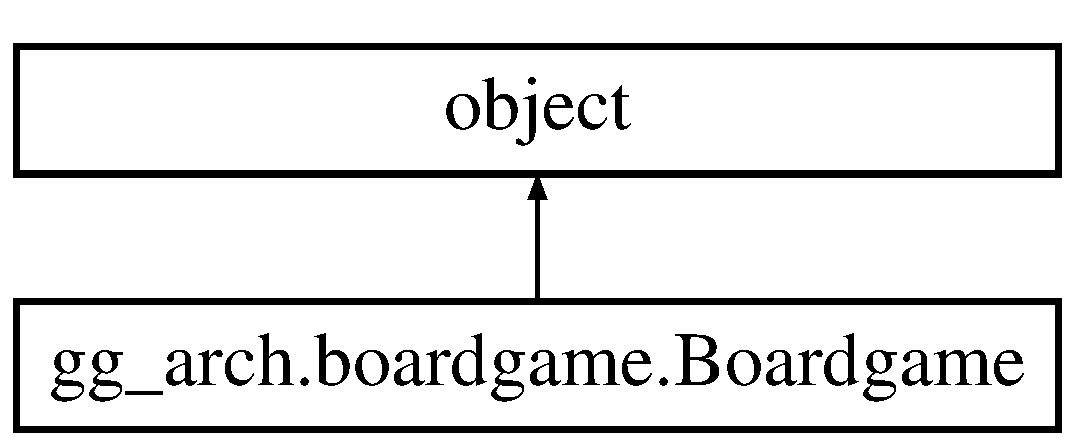
\includegraphics[height=2.000000cm]{classgg__arch_1_1boardgame_1_1_boardgame}
\end{center}
\end{figure}
\subsection*{Public Member Functions}
\begin{DoxyCompactItemize}
\item 
def \hyperlink{classgg__arch_1_1boardgame_1_1_boardgame_a9fabc6d25f2732b81c46c20fcc84890a}{\-\_\-\-\_\-init\-\_\-\-\_\-}
\item 
def \hyperlink{classgg__arch_1_1boardgame_1_1_boardgame_a241fc5e6df46e0a3b91214730e5ca7ca}{get\-Board}
\item 
def \hyperlink{classgg__arch_1_1boardgame_1_1_boardgame_ad09b9d93abd9c2ddbfb8f30cd3ba024f}{get\-History}
\item 
def \hyperlink{classgg__arch_1_1boardgame_1_1_boardgame_ac8990eebf22549f1ac0f1130414f4494}{make\-\_\-move}
\item 
def \hyperlink{classgg__arch_1_1boardgame_1_1_boardgame_a7918e8105d6d6978eb8b6b9f7a2aacf7}{get\-Cell\-Index}
\end{DoxyCompactItemize}
\subsection*{Static Public Attributes}
\begin{DoxyCompactItemize}
\item 
dictionary \hyperlink{classgg__arch_1_1boardgame_1_1_boardgame_a16f3034f66bd2ced22229b5798b8facc}{state} = \{\}
\item 
list \hyperlink{classgg__arch_1_1boardgame_1_1_boardgame_aba6edf60f3fe1db68ba0942b286f6db1}{history} = \mbox{[}$\,$\mbox{]}
\item 
list \hyperlink{classgg__arch_1_1boardgame_1_1_boardgame_a7425432d37ef9f90d9cc187f972c2052}{pieces} = \mbox{[}$\,$\mbox{]}
\item 
string \hyperlink{classgg__arch_1_1boardgame_1_1_boardgame_ad44b46bc2ec5b19f8139b76190d0768a}{boardtype} = ''
\item 
dictionary \hyperlink{classgg__arch_1_1boardgame_1_1_boardgame_a4abfdbb15a05a6278d9de43f54e46966}{board} = \{\}
\item 
int \hyperlink{classgg__arch_1_1boardgame_1_1_boardgame_a300c594f23db1b4c6659e23ec6304832}{num\-\_\-players} = 0
\end{DoxyCompactItemize}


\subsection{Detailed Description}
Copyright 2013 Hans Rinderknecht. 

This file is part of \hyperlink{namespacegg_player}{gg\-Player}. \hyperlink{namespacegg_player}{gg\-Player} is free software\-: you can redistribute it and/or modify it under the terms of the G\-N\-U General Public License as published by the Free Software Foundation, either version 3 of the License, or (at your option) any later version. \hyperlink{namespacegg_player}{gg\-Player} is distributed in the hope that it will be useful, but W\-I\-T\-H\-O\-U\-T A\-N\-Y W\-A\-R\-R\-A\-N\-T\-Y; without even the implied warranty of M\-E\-R\-C\-H\-A\-N\-T\-A\-B\-I\-L\-I\-T\-Y or F\-I\-T\-N\-E\-S\-S F\-O\-R A P\-A\-R\-T\-I\-C\-U\-L\-A\-R P\-U\-R\-P\-O\-S\-E. See the G\-N\-U General Public License for more details. You should have received a copy of the G\-N\-U General Public License along with \hyperlink{namespacegg_player}{gg\-Player}. If not, see \href{http://www.gnu.org/licenses/}{\tt http\-://www.\-gnu.\-org/licenses/}. \begin{DoxyVerb}Common boardgame class

This is an example of the basic class for a boardgame object.  Specific games (including boards, pieces, and rulesets) will be created as subclasses of this object.
\end{DoxyVerb}
 

\subsection{Constructor \& Destructor Documentation}
\hypertarget{classgg__arch_1_1boardgame_1_1_boardgame_a9fabc6d25f2732b81c46c20fcc84890a}{\index{gg\-\_\-arch\-::boardgame\-::\-Boardgame@{gg\-\_\-arch\-::boardgame\-::\-Boardgame}!\-\_\-\-\_\-init\-\_\-\-\_\-@{\-\_\-\-\_\-init\-\_\-\-\_\-}}
\index{\-\_\-\-\_\-init\-\_\-\-\_\-@{\-\_\-\-\_\-init\-\_\-\-\_\-}!gg_arch::boardgame::Boardgame@{gg\-\_\-arch\-::boardgame\-::\-Boardgame}}
\subsubsection[{\-\_\-\-\_\-init\-\_\-\-\_\-}]{\setlength{\rightskip}{0pt plus 5cm}def gg\-\_\-arch.\-boardgame.\-Boardgame.\-\_\-\-\_\-init\-\_\-\-\_\- (
\begin{DoxyParamCaption}
\item[{}]{self, }
\item[{}]{game}
\end{DoxyParamCaption}
)}}\label{classgg__arch_1_1boardgame_1_1_boardgame_a9fabc6d25f2732b81c46c20fcc84890a}


\subsection{Member Function Documentation}
\hypertarget{classgg__arch_1_1boardgame_1_1_boardgame_a241fc5e6df46e0a3b91214730e5ca7ca}{\index{gg\-\_\-arch\-::boardgame\-::\-Boardgame@{gg\-\_\-arch\-::boardgame\-::\-Boardgame}!get\-Board@{get\-Board}}
\index{get\-Board@{get\-Board}!gg_arch::boardgame::Boardgame@{gg\-\_\-arch\-::boardgame\-::\-Boardgame}}
\subsubsection[{get\-Board}]{\setlength{\rightskip}{0pt plus 5cm}def gg\-\_\-arch.\-boardgame.\-Boardgame.\-get\-Board (
\begin{DoxyParamCaption}
\item[{}]{self}
\end{DoxyParamCaption}
)}}\label{classgg__arch_1_1boardgame_1_1_boardgame_a241fc5e6df46e0a3b91214730e5ca7ca}
\begin{DoxyVerb}Initializes the boardgame object\end{DoxyVerb}
\begin{DoxyVerb}Return the current state of the board\end{DoxyVerb}
 \hypertarget{classgg__arch_1_1boardgame_1_1_boardgame_a7918e8105d6d6978eb8b6b9f7a2aacf7}{\index{gg\-\_\-arch\-::boardgame\-::\-Boardgame@{gg\-\_\-arch\-::boardgame\-::\-Boardgame}!get\-Cell\-Index@{get\-Cell\-Index}}
\index{get\-Cell\-Index@{get\-Cell\-Index}!gg_arch::boardgame::Boardgame@{gg\-\_\-arch\-::boardgame\-::\-Boardgame}}
\subsubsection[{get\-Cell\-Index}]{\setlength{\rightskip}{0pt plus 5cm}def gg\-\_\-arch.\-boardgame.\-Boardgame.\-get\-Cell\-Index (
\begin{DoxyParamCaption}
\item[{}]{self, }
\item[{}]{cell\-\_\-name}
\end{DoxyParamCaption}
)}}\label{classgg__arch_1_1boardgame_1_1_boardgame_a7918e8105d6d6978eb8b6b9f7a2aacf7}
\hypertarget{classgg__arch_1_1boardgame_1_1_boardgame_ad09b9d93abd9c2ddbfb8f30cd3ba024f}{\index{gg\-\_\-arch\-::boardgame\-::\-Boardgame@{gg\-\_\-arch\-::boardgame\-::\-Boardgame}!get\-History@{get\-History}}
\index{get\-History@{get\-History}!gg_arch::boardgame::Boardgame@{gg\-\_\-arch\-::boardgame\-::\-Boardgame}}
\subsubsection[{get\-History}]{\setlength{\rightskip}{0pt plus 5cm}def gg\-\_\-arch.\-boardgame.\-Boardgame.\-get\-History (
\begin{DoxyParamCaption}
\item[{}]{self}
\end{DoxyParamCaption}
)}}\label{classgg__arch_1_1boardgame_1_1_boardgame_ad09b9d93abd9c2ddbfb8f30cd3ba024f}
\begin{DoxyVerb}Return the history of executed moves\end{DoxyVerb}
 \hypertarget{classgg__arch_1_1boardgame_1_1_boardgame_ac8990eebf22549f1ac0f1130414f4494}{\index{gg\-\_\-arch\-::boardgame\-::\-Boardgame@{gg\-\_\-arch\-::boardgame\-::\-Boardgame}!make\-\_\-move@{make\-\_\-move}}
\index{make\-\_\-move@{make\-\_\-move}!gg_arch::boardgame::Boardgame@{gg\-\_\-arch\-::boardgame\-::\-Boardgame}}
\subsubsection[{make\-\_\-move}]{\setlength{\rightskip}{0pt plus 5cm}def gg\-\_\-arch.\-boardgame.\-Boardgame.\-make\-\_\-move (
\begin{DoxyParamCaption}
\item[{}]{self, }
\item[{}]{piece\-\_\-\-I\-D, }
\item[{}]{cell\-\_\-\-I\-D}
\end{DoxyParamCaption}
)}}\label{classgg__arch_1_1boardgame_1_1_boardgame_ac8990eebf22549f1ac0f1130414f4494}


\subsection{Member Data Documentation}
\hypertarget{classgg__arch_1_1boardgame_1_1_boardgame_a4abfdbb15a05a6278d9de43f54e46966}{\index{gg\-\_\-arch\-::boardgame\-::\-Boardgame@{gg\-\_\-arch\-::boardgame\-::\-Boardgame}!board@{board}}
\index{board@{board}!gg_arch::boardgame::Boardgame@{gg\-\_\-arch\-::boardgame\-::\-Boardgame}}
\subsubsection[{board}]{\setlength{\rightskip}{0pt plus 5cm}dictionary gg\-\_\-arch.\-boardgame.\-Boardgame.\-board = \{\}\hspace{0.3cm}{\ttfamily [static]}}}\label{classgg__arch_1_1boardgame_1_1_boardgame_a4abfdbb15a05a6278d9de43f54e46966}
\hypertarget{classgg__arch_1_1boardgame_1_1_boardgame_ad44b46bc2ec5b19f8139b76190d0768a}{\index{gg\-\_\-arch\-::boardgame\-::\-Boardgame@{gg\-\_\-arch\-::boardgame\-::\-Boardgame}!boardtype@{boardtype}}
\index{boardtype@{boardtype}!gg_arch::boardgame::Boardgame@{gg\-\_\-arch\-::boardgame\-::\-Boardgame}}
\subsubsection[{boardtype}]{\setlength{\rightskip}{0pt plus 5cm}string gg\-\_\-arch.\-boardgame.\-Boardgame.\-boardtype = ''\hspace{0.3cm}{\ttfamily [static]}}}\label{classgg__arch_1_1boardgame_1_1_boardgame_ad44b46bc2ec5b19f8139b76190d0768a}
\hypertarget{classgg__arch_1_1boardgame_1_1_boardgame_aba6edf60f3fe1db68ba0942b286f6db1}{\index{gg\-\_\-arch\-::boardgame\-::\-Boardgame@{gg\-\_\-arch\-::boardgame\-::\-Boardgame}!history@{history}}
\index{history@{history}!gg_arch::boardgame::Boardgame@{gg\-\_\-arch\-::boardgame\-::\-Boardgame}}
\subsubsection[{history}]{\setlength{\rightskip}{0pt plus 5cm}list gg\-\_\-arch.\-boardgame.\-Boardgame.\-history = \mbox{[}$\,$\mbox{]}\hspace{0.3cm}{\ttfamily [static]}}}\label{classgg__arch_1_1boardgame_1_1_boardgame_aba6edf60f3fe1db68ba0942b286f6db1}
\hypertarget{classgg__arch_1_1boardgame_1_1_boardgame_a300c594f23db1b4c6659e23ec6304832}{\index{gg\-\_\-arch\-::boardgame\-::\-Boardgame@{gg\-\_\-arch\-::boardgame\-::\-Boardgame}!num\-\_\-players@{num\-\_\-players}}
\index{num\-\_\-players@{num\-\_\-players}!gg_arch::boardgame::Boardgame@{gg\-\_\-arch\-::boardgame\-::\-Boardgame}}
\subsubsection[{num\-\_\-players}]{\setlength{\rightskip}{0pt plus 5cm}int gg\-\_\-arch.\-boardgame.\-Boardgame.\-num\-\_\-players = 0\hspace{0.3cm}{\ttfamily [static]}}}\label{classgg__arch_1_1boardgame_1_1_boardgame_a300c594f23db1b4c6659e23ec6304832}
\hypertarget{classgg__arch_1_1boardgame_1_1_boardgame_a7425432d37ef9f90d9cc187f972c2052}{\index{gg\-\_\-arch\-::boardgame\-::\-Boardgame@{gg\-\_\-arch\-::boardgame\-::\-Boardgame}!pieces@{pieces}}
\index{pieces@{pieces}!gg_arch::boardgame::Boardgame@{gg\-\_\-arch\-::boardgame\-::\-Boardgame}}
\subsubsection[{pieces}]{\setlength{\rightskip}{0pt plus 5cm}list gg\-\_\-arch.\-boardgame.\-Boardgame.\-pieces = \mbox{[}$\,$\mbox{]}\hspace{0.3cm}{\ttfamily [static]}}}\label{classgg__arch_1_1boardgame_1_1_boardgame_a7425432d37ef9f90d9cc187f972c2052}
\hypertarget{classgg__arch_1_1boardgame_1_1_boardgame_a16f3034f66bd2ced22229b5798b8facc}{\index{gg\-\_\-arch\-::boardgame\-::\-Boardgame@{gg\-\_\-arch\-::boardgame\-::\-Boardgame}!state@{state}}
\index{state@{state}!gg_arch::boardgame::Boardgame@{gg\-\_\-arch\-::boardgame\-::\-Boardgame}}
\subsubsection[{state}]{\setlength{\rightskip}{0pt plus 5cm}dictionary gg\-\_\-arch.\-boardgame.\-Boardgame.\-state = \{\}\hspace{0.3cm}{\ttfamily [static]}}}\label{classgg__arch_1_1boardgame_1_1_boardgame_a16f3034f66bd2ced22229b5798b8facc}


The documentation for this class was generated from the following file\-:\begin{DoxyCompactItemize}
\item 
gg\-\_\-arch/\hyperlink{boardgame_8py}{boardgame.\-py}\end{DoxyCompactItemize}

\hypertarget{classgg__arch_1_1chess_1_1_chess}{\section{gg\-\_\-arch.\-chess.\-Chess Class Reference}
\label{classgg__arch_1_1chess_1_1_chess}\index{gg\-\_\-arch.\-chess.\-Chess@{gg\-\_\-arch.\-chess.\-Chess}}
}
Inheritance diagram for gg\-\_\-arch.\-chess.\-Chess\-:\begin{figure}[H]
\begin{center}
\leavevmode
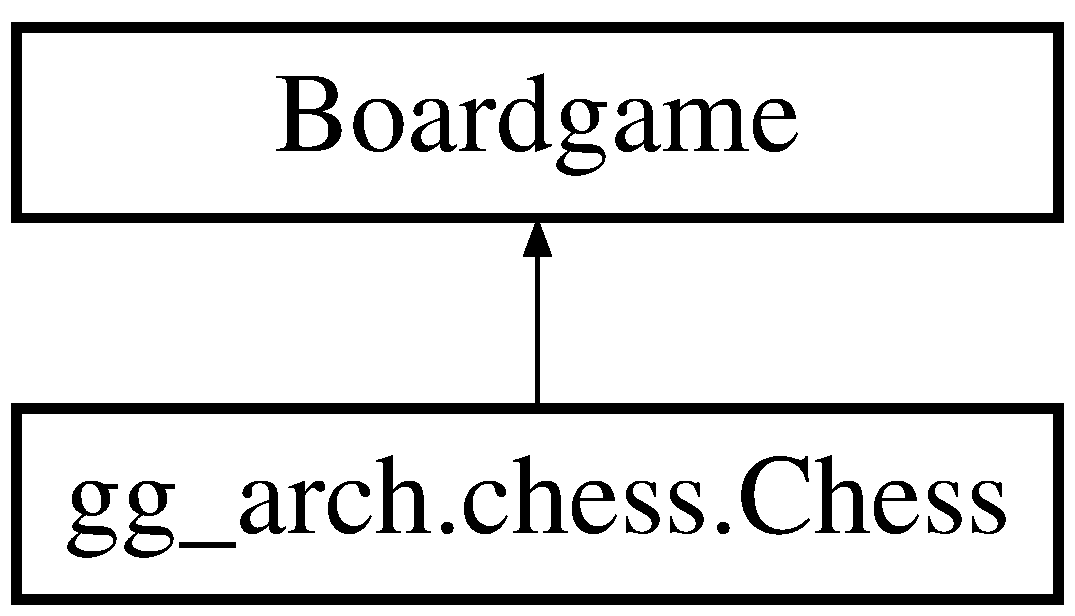
\includegraphics[height=2.000000cm]{classgg__arch_1_1chess_1_1_chess}
\end{center}
\end{figure}
\subsection*{Public Member Functions}
\begin{DoxyCompactItemize}
\item 
def \hyperlink{classgg__arch_1_1chess_1_1_chess_a2a82d2e17e698e72edbf8183b9e4a013}{\-\_\-\-\_\-init\-\_\-\-\_\-}
\end{DoxyCompactItemize}
\subsection*{Public Attributes}
\begin{DoxyCompactItemize}
\item 
\hyperlink{classgg__arch_1_1chess_1_1_chess_ad01e5c1a7c3416cab1f5b1b9cc22ea58}{pieces}
\end{DoxyCompactItemize}
\subsection*{Static Public Attributes}
\begin{DoxyCompactItemize}
\item 
string \hyperlink{classgg__arch_1_1chess_1_1_chess_aa82ec766cebfa6d144948a71f1dcf0d3}{boardtype} = '8x8checker'
\item 
int \hyperlink{classgg__arch_1_1chess_1_1_chess_a8d218ad53b70be5163ddeb252c144c70}{num\-\_\-players} = 2
\end{DoxyCompactItemize}


\subsection{Constructor \& Destructor Documentation}
\hypertarget{classgg__arch_1_1chess_1_1_chess_a2a82d2e17e698e72edbf8183b9e4a013}{\index{gg\-\_\-arch\-::chess\-::\-Chess@{gg\-\_\-arch\-::chess\-::\-Chess}!\-\_\-\-\_\-init\-\_\-\-\_\-@{\-\_\-\-\_\-init\-\_\-\-\_\-}}
\index{\-\_\-\-\_\-init\-\_\-\-\_\-@{\-\_\-\-\_\-init\-\_\-\-\_\-}!gg_arch::chess::Chess@{gg\-\_\-arch\-::chess\-::\-Chess}}
\subsubsection[{\-\_\-\-\_\-init\-\_\-\-\_\-}]{\setlength{\rightskip}{0pt plus 5cm}def gg\-\_\-arch.\-chess.\-Chess.\-\_\-\-\_\-init\-\_\-\-\_\- (
\begin{DoxyParamCaption}
\item[{}]{self}
\end{DoxyParamCaption}
)}}\label{classgg__arch_1_1chess_1_1_chess_a2a82d2e17e698e72edbf8183b9e4a013}


\subsection{Member Data Documentation}
\hypertarget{classgg__arch_1_1chess_1_1_chess_aa82ec766cebfa6d144948a71f1dcf0d3}{\index{gg\-\_\-arch\-::chess\-::\-Chess@{gg\-\_\-arch\-::chess\-::\-Chess}!boardtype@{boardtype}}
\index{boardtype@{boardtype}!gg_arch::chess::Chess@{gg\-\_\-arch\-::chess\-::\-Chess}}
\subsubsection[{boardtype}]{\setlength{\rightskip}{0pt plus 5cm}string gg\-\_\-arch.\-chess.\-Chess.\-boardtype = '8x8checker'\hspace{0.3cm}{\ttfamily [static]}}}\label{classgg__arch_1_1chess_1_1_chess_aa82ec766cebfa6d144948a71f1dcf0d3}
\hypertarget{classgg__arch_1_1chess_1_1_chess_a8d218ad53b70be5163ddeb252c144c70}{\index{gg\-\_\-arch\-::chess\-::\-Chess@{gg\-\_\-arch\-::chess\-::\-Chess}!num\-\_\-players@{num\-\_\-players}}
\index{num\-\_\-players@{num\-\_\-players}!gg_arch::chess::Chess@{gg\-\_\-arch\-::chess\-::\-Chess}}
\subsubsection[{num\-\_\-players}]{\setlength{\rightskip}{0pt plus 5cm}int gg\-\_\-arch.\-chess.\-Chess.\-num\-\_\-players = 2\hspace{0.3cm}{\ttfamily [static]}}}\label{classgg__arch_1_1chess_1_1_chess_a8d218ad53b70be5163ddeb252c144c70}
\hypertarget{classgg__arch_1_1chess_1_1_chess_ad01e5c1a7c3416cab1f5b1b9cc22ea58}{\index{gg\-\_\-arch\-::chess\-::\-Chess@{gg\-\_\-arch\-::chess\-::\-Chess}!pieces@{pieces}}
\index{pieces@{pieces}!gg_arch::chess::Chess@{gg\-\_\-arch\-::chess\-::\-Chess}}
\subsubsection[{pieces}]{\setlength{\rightskip}{0pt plus 5cm}gg\-\_\-arch.\-chess.\-Chess.\-pieces}}\label{classgg__arch_1_1chess_1_1_chess_ad01e5c1a7c3416cab1f5b1b9cc22ea58}


The documentation for this class was generated from the following file\-:\begin{DoxyCompactItemize}
\item 
gg\-\_\-arch/\hyperlink{chess_8py}{chess.\-py}\end{DoxyCompactItemize}

\hypertarget{classgg_player_1_1_game_canvas}{\section{gg\-Player.\-Game\-Canvas Class Reference}
\label{classgg_player_1_1_game_canvas}\index{gg\-Player.\-Game\-Canvas@{gg\-Player.\-Game\-Canvas}}
}
Inheritance diagram for gg\-Player.\-Game\-Canvas\-:\begin{figure}[H]
\begin{center}
\leavevmode
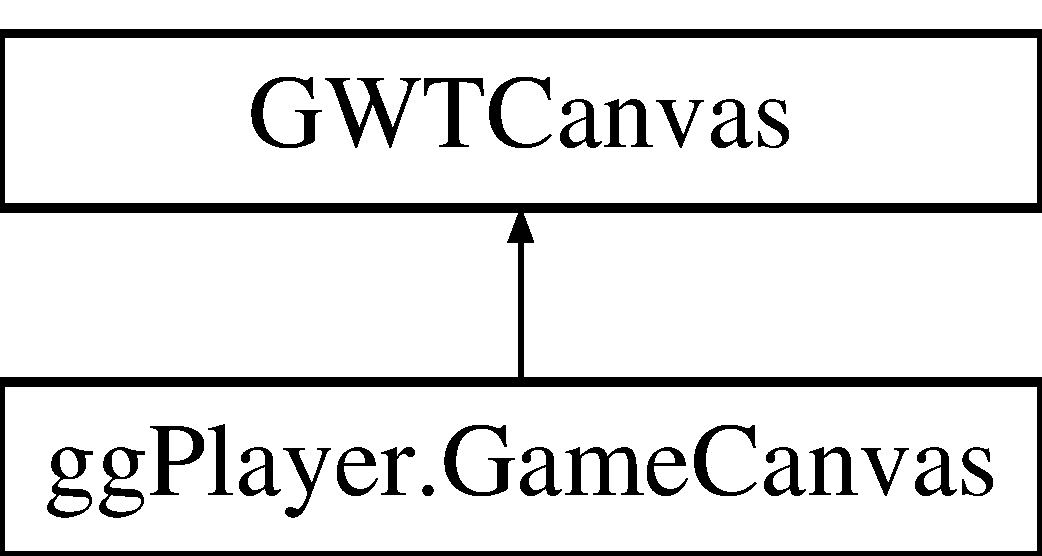
\includegraphics[height=2.000000cm]{classgg_player_1_1_game_canvas}
\end{center}
\end{figure}
\subsection*{Public Member Functions}
\begin{DoxyCompactItemize}
\item 
def \hyperlink{classgg_player_1_1_game_canvas_ac35576177ebfe767f36defa0860f0c7c}{\-\_\-\-\_\-init\-\_\-\-\_\-}
\item 
def \hyperlink{classgg_player_1_1_game_canvas_aefb06840926a20f3cc47c23f18aee269}{load\-Game}
\item 
def \hyperlink{classgg_player_1_1_game_canvas_a7389e112bc0cab38e3cbe836dd65004b}{on\-Images\-Loaded}
\item 
def \hyperlink{classgg_player_1_1_game_canvas_ad4261b18fb7ef9fa0e4b2c8b6b1c0a6f}{reset}
\item 
def \hyperlink{classgg_player_1_1_game_canvas_a49a36f712bddfe3ec15b4002560f027d}{draw\-Board}
\end{DoxyCompactItemize}
\subsection*{Public Attributes}
\begin{DoxyCompactItemize}
\item 
\hyperlink{classgg_player_1_1_game_canvas_aa8882a242adc63c849416b7b558dc2f8}{width}
\item 
\hyperlink{classgg_player_1_1_game_canvas_a801eb36c0f8fb9927b6843263243d49b}{height}
\item 
\hyperlink{classgg_player_1_1_game_canvas_a383c5decaed718ccdaccba538aba8194}{gametype}
\item 
\hyperlink{classgg_player_1_1_game_canvas_ad2337a4445e3a20847859f101e83fe4c}{images}
\item 
\hyperlink{classgg_player_1_1_game_canvas_ade98cc3308349102b56503d9e3315dc3}{img\-\_\-dict}
\item 
\hyperlink{classgg_player_1_1_game_canvas_a2313c2d189e08686e0b3ecbbf6c3c6b0}{run}
\item 
\hyperlink{classgg_player_1_1_game_canvas_a6bdab1f0c4b24247652cbe9fb4cff376}{game}
\item 
\hyperlink{classgg_player_1_1_game_canvas_aa9121cb6ed54defa6ddd26b141bd9ea3}{boardtype}
\end{DoxyCompactItemize}


\subsection{Constructor \& Destructor Documentation}
\hypertarget{classgg_player_1_1_game_canvas_ac35576177ebfe767f36defa0860f0c7c}{\index{gg\-Player\-::\-Game\-Canvas@{gg\-Player\-::\-Game\-Canvas}!\-\_\-\-\_\-init\-\_\-\-\_\-@{\-\_\-\-\_\-init\-\_\-\-\_\-}}
\index{\-\_\-\-\_\-init\-\_\-\-\_\-@{\-\_\-\-\_\-init\-\_\-\-\_\-}!ggPlayer::GameCanvas@{gg\-Player\-::\-Game\-Canvas}}
\subsubsection[{\-\_\-\-\_\-init\-\_\-\-\_\-}]{\setlength{\rightskip}{0pt plus 5cm}def gg\-Player.\-Game\-Canvas.\-\_\-\-\_\-init\-\_\-\-\_\- (
\begin{DoxyParamCaption}
\item[{}]{self, }
\item[{}]{w, }
\item[{}]{h, }
\item[{}]{gametype}
\end{DoxyParamCaption}
)}}\label{classgg_player_1_1_game_canvas_ac35576177ebfe767f36defa0860f0c7c}


\subsection{Member Function Documentation}
\hypertarget{classgg_player_1_1_game_canvas_a49a36f712bddfe3ec15b4002560f027d}{\index{gg\-Player\-::\-Game\-Canvas@{gg\-Player\-::\-Game\-Canvas}!draw\-Board@{draw\-Board}}
\index{draw\-Board@{draw\-Board}!ggPlayer::GameCanvas@{gg\-Player\-::\-Game\-Canvas}}
\subsubsection[{draw\-Board}]{\setlength{\rightskip}{0pt plus 5cm}def gg\-Player.\-Game\-Canvas.\-draw\-Board (
\begin{DoxyParamCaption}
\item[{}]{self}
\end{DoxyParamCaption}
)}}\label{classgg_player_1_1_game_canvas_a49a36f712bddfe3ec15b4002560f027d}
\hypertarget{classgg_player_1_1_game_canvas_aefb06840926a20f3cc47c23f18aee269}{\index{gg\-Player\-::\-Game\-Canvas@{gg\-Player\-::\-Game\-Canvas}!load\-Game@{load\-Game}}
\index{load\-Game@{load\-Game}!ggPlayer::GameCanvas@{gg\-Player\-::\-Game\-Canvas}}
\subsubsection[{load\-Game}]{\setlength{\rightskip}{0pt plus 5cm}def gg\-Player.\-Game\-Canvas.\-load\-Game (
\begin{DoxyParamCaption}
\item[{}]{self}
\end{DoxyParamCaption}
)}}\label{classgg_player_1_1_game_canvas_aefb06840926a20f3cc47c23f18aee269}
\hypertarget{classgg_player_1_1_game_canvas_a7389e112bc0cab38e3cbe836dd65004b}{\index{gg\-Player\-::\-Game\-Canvas@{gg\-Player\-::\-Game\-Canvas}!on\-Images\-Loaded@{on\-Images\-Loaded}}
\index{on\-Images\-Loaded@{on\-Images\-Loaded}!ggPlayer::GameCanvas@{gg\-Player\-::\-Game\-Canvas}}
\subsubsection[{on\-Images\-Loaded}]{\setlength{\rightskip}{0pt plus 5cm}def gg\-Player.\-Game\-Canvas.\-on\-Images\-Loaded (
\begin{DoxyParamCaption}
\item[{}]{self, }
\item[{}]{images\-Handles}
\end{DoxyParamCaption}
)}}\label{classgg_player_1_1_game_canvas_a7389e112bc0cab38e3cbe836dd65004b}
\hypertarget{classgg_player_1_1_game_canvas_ad4261b18fb7ef9fa0e4b2c8b6b1c0a6f}{\index{gg\-Player\-::\-Game\-Canvas@{gg\-Player\-::\-Game\-Canvas}!reset@{reset}}
\index{reset@{reset}!ggPlayer::GameCanvas@{gg\-Player\-::\-Game\-Canvas}}
\subsubsection[{reset}]{\setlength{\rightskip}{0pt plus 5cm}def gg\-Player.\-Game\-Canvas.\-reset (
\begin{DoxyParamCaption}
\item[{}]{self}
\end{DoxyParamCaption}
)}}\label{classgg_player_1_1_game_canvas_ad4261b18fb7ef9fa0e4b2c8b6b1c0a6f}


\subsection{Member Data Documentation}
\hypertarget{classgg_player_1_1_game_canvas_aa9121cb6ed54defa6ddd26b141bd9ea3}{\index{gg\-Player\-::\-Game\-Canvas@{gg\-Player\-::\-Game\-Canvas}!boardtype@{boardtype}}
\index{boardtype@{boardtype}!ggPlayer::GameCanvas@{gg\-Player\-::\-Game\-Canvas}}
\subsubsection[{boardtype}]{\setlength{\rightskip}{0pt plus 5cm}gg\-Player.\-Game\-Canvas.\-boardtype}}\label{classgg_player_1_1_game_canvas_aa9121cb6ed54defa6ddd26b141bd9ea3}
\hypertarget{classgg_player_1_1_game_canvas_a6bdab1f0c4b24247652cbe9fb4cff376}{\index{gg\-Player\-::\-Game\-Canvas@{gg\-Player\-::\-Game\-Canvas}!game@{game}}
\index{game@{game}!ggPlayer::GameCanvas@{gg\-Player\-::\-Game\-Canvas}}
\subsubsection[{game}]{\setlength{\rightskip}{0pt plus 5cm}gg\-Player.\-Game\-Canvas.\-game}}\label{classgg_player_1_1_game_canvas_a6bdab1f0c4b24247652cbe9fb4cff376}
\hypertarget{classgg_player_1_1_game_canvas_a383c5decaed718ccdaccba538aba8194}{\index{gg\-Player\-::\-Game\-Canvas@{gg\-Player\-::\-Game\-Canvas}!gametype@{gametype}}
\index{gametype@{gametype}!ggPlayer::GameCanvas@{gg\-Player\-::\-Game\-Canvas}}
\subsubsection[{gametype}]{\setlength{\rightskip}{0pt plus 5cm}gg\-Player.\-Game\-Canvas.\-gametype}}\label{classgg_player_1_1_game_canvas_a383c5decaed718ccdaccba538aba8194}
\hypertarget{classgg_player_1_1_game_canvas_a801eb36c0f8fb9927b6843263243d49b}{\index{gg\-Player\-::\-Game\-Canvas@{gg\-Player\-::\-Game\-Canvas}!height@{height}}
\index{height@{height}!ggPlayer::GameCanvas@{gg\-Player\-::\-Game\-Canvas}}
\subsubsection[{height}]{\setlength{\rightskip}{0pt plus 5cm}gg\-Player.\-Game\-Canvas.\-height}}\label{classgg_player_1_1_game_canvas_a801eb36c0f8fb9927b6843263243d49b}
\hypertarget{classgg_player_1_1_game_canvas_ad2337a4445e3a20847859f101e83fe4c}{\index{gg\-Player\-::\-Game\-Canvas@{gg\-Player\-::\-Game\-Canvas}!images@{images}}
\index{images@{images}!ggPlayer::GameCanvas@{gg\-Player\-::\-Game\-Canvas}}
\subsubsection[{images}]{\setlength{\rightskip}{0pt plus 5cm}gg\-Player.\-Game\-Canvas.\-images}}\label{classgg_player_1_1_game_canvas_ad2337a4445e3a20847859f101e83fe4c}
\hypertarget{classgg_player_1_1_game_canvas_ade98cc3308349102b56503d9e3315dc3}{\index{gg\-Player\-::\-Game\-Canvas@{gg\-Player\-::\-Game\-Canvas}!img\-\_\-dict@{img\-\_\-dict}}
\index{img\-\_\-dict@{img\-\_\-dict}!ggPlayer::GameCanvas@{gg\-Player\-::\-Game\-Canvas}}
\subsubsection[{img\-\_\-dict}]{\setlength{\rightskip}{0pt plus 5cm}gg\-Player.\-Game\-Canvas.\-img\-\_\-dict}}\label{classgg_player_1_1_game_canvas_ade98cc3308349102b56503d9e3315dc3}
\hypertarget{classgg_player_1_1_game_canvas_a2313c2d189e08686e0b3ecbbf6c3c6b0}{\index{gg\-Player\-::\-Game\-Canvas@{gg\-Player\-::\-Game\-Canvas}!run@{run}}
\index{run@{run}!ggPlayer::GameCanvas@{gg\-Player\-::\-Game\-Canvas}}
\subsubsection[{run}]{\setlength{\rightskip}{0pt plus 5cm}gg\-Player.\-Game\-Canvas.\-run}}\label{classgg_player_1_1_game_canvas_a2313c2d189e08686e0b3ecbbf6c3c6b0}
\hypertarget{classgg_player_1_1_game_canvas_aa8882a242adc63c849416b7b558dc2f8}{\index{gg\-Player\-::\-Game\-Canvas@{gg\-Player\-::\-Game\-Canvas}!width@{width}}
\index{width@{width}!ggPlayer::GameCanvas@{gg\-Player\-::\-Game\-Canvas}}
\subsubsection[{width}]{\setlength{\rightskip}{0pt plus 5cm}gg\-Player.\-Game\-Canvas.\-width}}\label{classgg_player_1_1_game_canvas_aa8882a242adc63c849416b7b558dc2f8}


The documentation for this class was generated from the following file\-:\begin{DoxyCompactItemize}
\item 
ggplayer/\hyperlink{gg_player_8py}{gg\-Player.\-py}\end{DoxyCompactItemize}

\hypertarget{classgg__arch_1_1gamecell_1_1game_cell}{\section{gg\-\_\-arch.\-gamecell.\-game\-Cell Class Reference}
\label{classgg__arch_1_1gamecell_1_1game_cell}\index{gg\-\_\-arch.\-gamecell.\-game\-Cell@{gg\-\_\-arch.\-gamecell.\-game\-Cell}}
}


Copyright 2013 Hans Rinderknecht.  


Inheritance diagram for gg\-\_\-arch.\-gamecell.\-game\-Cell\-:\begin{figure}[H]
\begin{center}
\leavevmode
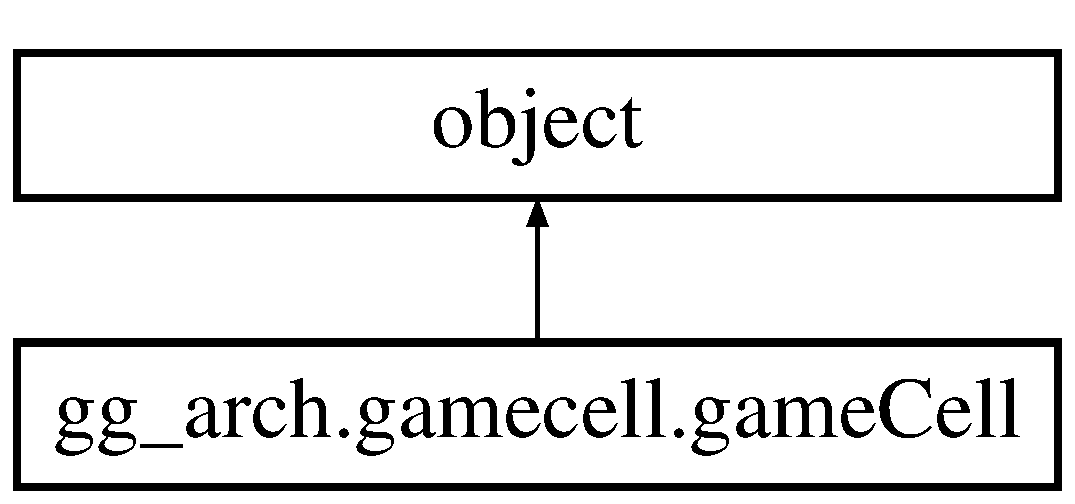
\includegraphics[height=2.000000cm]{classgg__arch_1_1gamecell_1_1game_cell}
\end{center}
\end{figure}
\subsection*{Public Member Functions}
\begin{DoxyCompactItemize}
\item 
def \hyperlink{classgg__arch_1_1gamecell_1_1game_cell_ab8530cca4fbeecff3c0c640a9a54d1a5}{\-\_\-\-\_\-init\-\_\-\-\_\-}
\item 
def \hyperlink{classgg__arch_1_1gamecell_1_1game_cell_a9e3e51533b4e4c218d0797594eca21bc}{get\-Path}
\item 
def \hyperlink{classgg__arch_1_1gamecell_1_1game_cell_a871fbb9dac6b5417d36bcf5d67ff7450}{get\-Pos}
\item 
def \hyperlink{classgg__arch_1_1gamecell_1_1game_cell_af252d35279981de75c47dd5ba9c71a63}{get\-Size}
\end{DoxyCompactItemize}
\subsection*{Public Attributes}
\begin{DoxyCompactItemize}
\item 
\hyperlink{classgg__arch_1_1gamecell_1_1game_cell_ada75b7dbbea4a61dc10b6227a43d0f78}{name}
\item 
\hyperlink{classgg__arch_1_1gamecell_1_1game_cell_a68355a86a7580f16ade2446991f2a4b3}{shape}
\item 
\hyperlink{classgg__arch_1_1gamecell_1_1game_cell_aae0a2c4e1e821fee5c4d6d298840e403}{params}
\item 
\hyperlink{classgg__arch_1_1gamecell_1_1game_cell_ae87be21f16d1f9d0225e4826ccd46e1b}{color}
\end{DoxyCompactItemize}


\subsection{Detailed Description}
Copyright 2013 Hans Rinderknecht. 

This file is part of \hyperlink{namespacegg_player}{gg\-Player}. \hyperlink{namespacegg_player}{gg\-Player} is free software\-: you can redistribute it and/or modify it under the terms of the G\-N\-U General Public License as published by the Free Software Foundation, either version 3 of the License, or (at your option) any later version. \hyperlink{namespacegg_player}{gg\-Player} is distributed in the hope that it will be useful, but W\-I\-T\-H\-O\-U\-T A\-N\-Y W\-A\-R\-R\-A\-N\-T\-Y; without even the implied warranty of M\-E\-R\-C\-H\-A\-N\-T\-A\-B\-I\-L\-I\-T\-Y or F\-I\-T\-N\-E\-S\-S F\-O\-R A P\-A\-R\-T\-I\-C\-U\-L\-A\-R P\-U\-R\-P\-O\-S\-E. See the G\-N\-U General Public License for more details. You should have received a copy of the G\-N\-U General Public License along with \hyperlink{namespacegg_player}{gg\-Player}. If not, see \href{http://www.gnu.org/licenses/}{\tt http\-://www.\-gnu.\-org/licenses/}. \begin{DoxyVerb}Common game cell object.  [x,y] and [width, height] are fractions of the canvas size.\end{DoxyVerb}
 

\subsection{Constructor \& Destructor Documentation}
\hypertarget{classgg__arch_1_1gamecell_1_1game_cell_ab8530cca4fbeecff3c0c640a9a54d1a5}{\index{gg\-\_\-arch\-::gamecell\-::game\-Cell@{gg\-\_\-arch\-::gamecell\-::game\-Cell}!\-\_\-\-\_\-init\-\_\-\-\_\-@{\-\_\-\-\_\-init\-\_\-\-\_\-}}
\index{\-\_\-\-\_\-init\-\_\-\-\_\-@{\-\_\-\-\_\-init\-\_\-\-\_\-}!gg_arch::gamecell::gameCell@{gg\-\_\-arch\-::gamecell\-::game\-Cell}}
\subsubsection[{\-\_\-\-\_\-init\-\_\-\-\_\-}]{\setlength{\rightskip}{0pt plus 5cm}def gg\-\_\-arch.\-gamecell.\-game\-Cell.\-\_\-\-\_\-init\-\_\-\-\_\- (
\begin{DoxyParamCaption}
\item[{}]{self, }
\item[{}]{name, }
\item[{}]{color, }
\item[{}]{shape = {\ttfamily 'rect'}, }
\item[{}]{params = {\ttfamily \mbox{[}0}}
\end{DoxyParamCaption}
)}}\label{classgg__arch_1_1gamecell_1_1game_cell_ab8530cca4fbeecff3c0c640a9a54d1a5}


\subsection{Member Function Documentation}
\hypertarget{classgg__arch_1_1gamecell_1_1game_cell_a9e3e51533b4e4c218d0797594eca21bc}{\index{gg\-\_\-arch\-::gamecell\-::game\-Cell@{gg\-\_\-arch\-::gamecell\-::game\-Cell}!get\-Path@{get\-Path}}
\index{get\-Path@{get\-Path}!gg_arch::gamecell::gameCell@{gg\-\_\-arch\-::gamecell\-::game\-Cell}}
\subsubsection[{get\-Path}]{\setlength{\rightskip}{0pt plus 5cm}def gg\-\_\-arch.\-gamecell.\-game\-Cell.\-get\-Path (
\begin{DoxyParamCaption}
\item[{}]{self}
\end{DoxyParamCaption}
)}}\label{classgg__arch_1_1gamecell_1_1game_cell_a9e3e51533b4e4c218d0797594eca21bc}
\hypertarget{classgg__arch_1_1gamecell_1_1game_cell_a871fbb9dac6b5417d36bcf5d67ff7450}{\index{gg\-\_\-arch\-::gamecell\-::game\-Cell@{gg\-\_\-arch\-::gamecell\-::game\-Cell}!get\-Pos@{get\-Pos}}
\index{get\-Pos@{get\-Pos}!gg_arch::gamecell::gameCell@{gg\-\_\-arch\-::gamecell\-::game\-Cell}}
\subsubsection[{get\-Pos}]{\setlength{\rightskip}{0pt plus 5cm}def gg\-\_\-arch.\-gamecell.\-game\-Cell.\-get\-Pos (
\begin{DoxyParamCaption}
\item[{}]{self}
\end{DoxyParamCaption}
)}}\label{classgg__arch_1_1gamecell_1_1game_cell_a871fbb9dac6b5417d36bcf5d67ff7450}
\hypertarget{classgg__arch_1_1gamecell_1_1game_cell_af252d35279981de75c47dd5ba9c71a63}{\index{gg\-\_\-arch\-::gamecell\-::game\-Cell@{gg\-\_\-arch\-::gamecell\-::game\-Cell}!get\-Size@{get\-Size}}
\index{get\-Size@{get\-Size}!gg_arch::gamecell::gameCell@{gg\-\_\-arch\-::gamecell\-::game\-Cell}}
\subsubsection[{get\-Size}]{\setlength{\rightskip}{0pt plus 5cm}def gg\-\_\-arch.\-gamecell.\-game\-Cell.\-get\-Size (
\begin{DoxyParamCaption}
\item[{}]{self}
\end{DoxyParamCaption}
)}}\label{classgg__arch_1_1gamecell_1_1game_cell_af252d35279981de75c47dd5ba9c71a63}


\subsection{Member Data Documentation}
\hypertarget{classgg__arch_1_1gamecell_1_1game_cell_ae87be21f16d1f9d0225e4826ccd46e1b}{\index{gg\-\_\-arch\-::gamecell\-::game\-Cell@{gg\-\_\-arch\-::gamecell\-::game\-Cell}!color@{color}}
\index{color@{color}!gg_arch::gamecell::gameCell@{gg\-\_\-arch\-::gamecell\-::game\-Cell}}
\subsubsection[{color}]{\setlength{\rightskip}{0pt plus 5cm}gg\-\_\-arch.\-gamecell.\-game\-Cell.\-color}}\label{classgg__arch_1_1gamecell_1_1game_cell_ae87be21f16d1f9d0225e4826ccd46e1b}
\hypertarget{classgg__arch_1_1gamecell_1_1game_cell_ada75b7dbbea4a61dc10b6227a43d0f78}{\index{gg\-\_\-arch\-::gamecell\-::game\-Cell@{gg\-\_\-arch\-::gamecell\-::game\-Cell}!name@{name}}
\index{name@{name}!gg_arch::gamecell::gameCell@{gg\-\_\-arch\-::gamecell\-::game\-Cell}}
\subsubsection[{name}]{\setlength{\rightskip}{0pt plus 5cm}gg\-\_\-arch.\-gamecell.\-game\-Cell.\-name}}\label{classgg__arch_1_1gamecell_1_1game_cell_ada75b7dbbea4a61dc10b6227a43d0f78}
\hypertarget{classgg__arch_1_1gamecell_1_1game_cell_aae0a2c4e1e821fee5c4d6d298840e403}{\index{gg\-\_\-arch\-::gamecell\-::game\-Cell@{gg\-\_\-arch\-::gamecell\-::game\-Cell}!params@{params}}
\index{params@{params}!gg_arch::gamecell::gameCell@{gg\-\_\-arch\-::gamecell\-::game\-Cell}}
\subsubsection[{params}]{\setlength{\rightskip}{0pt plus 5cm}gg\-\_\-arch.\-gamecell.\-game\-Cell.\-params}}\label{classgg__arch_1_1gamecell_1_1game_cell_aae0a2c4e1e821fee5c4d6d298840e403}
\hypertarget{classgg__arch_1_1gamecell_1_1game_cell_a68355a86a7580f16ade2446991f2a4b3}{\index{gg\-\_\-arch\-::gamecell\-::game\-Cell@{gg\-\_\-arch\-::gamecell\-::game\-Cell}!shape@{shape}}
\index{shape@{shape}!gg_arch::gamecell::gameCell@{gg\-\_\-arch\-::gamecell\-::game\-Cell}}
\subsubsection[{shape}]{\setlength{\rightskip}{0pt plus 5cm}gg\-\_\-arch.\-gamecell.\-game\-Cell.\-shape}}\label{classgg__arch_1_1gamecell_1_1game_cell_a68355a86a7580f16ade2446991f2a4b3}


The documentation for this class was generated from the following file\-:\begin{DoxyCompactItemize}
\item 
gg\-\_\-arch/\hyperlink{gamecell_8py}{gamecell.\-py}\end{DoxyCompactItemize}

\hypertarget{classgg__arch_1_1gamepiece_1_1_gamepiece}{\section{gg\-\_\-arch.\-gamepiece.\-Gamepiece Class Reference}
\label{classgg__arch_1_1gamepiece_1_1_gamepiece}\index{gg\-\_\-arch.\-gamepiece.\-Gamepiece@{gg\-\_\-arch.\-gamepiece.\-Gamepiece}}
}


Copyright 2013 Hans Rinderknecht.  


Inheritance diagram for gg\-\_\-arch.\-gamepiece.\-Gamepiece\-:\begin{figure}[H]
\begin{center}
\leavevmode
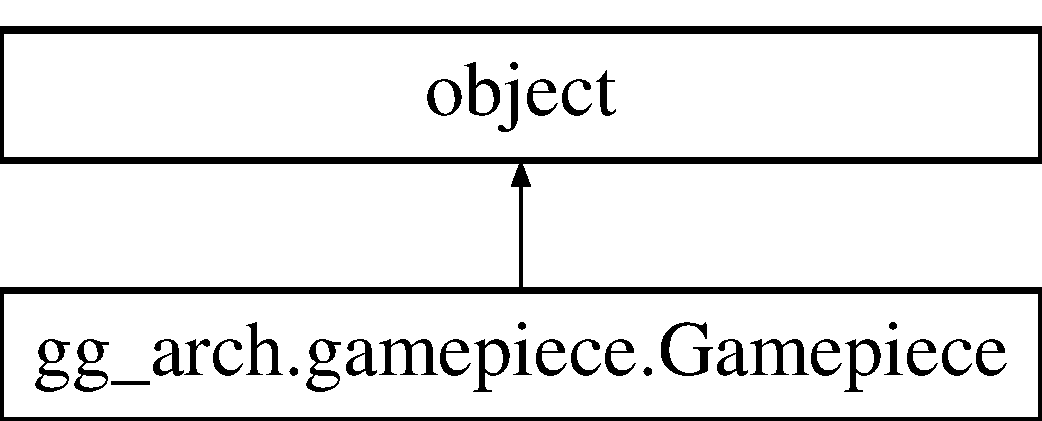
\includegraphics[height=2.000000cm]{classgg__arch_1_1gamepiece_1_1_gamepiece}
\end{center}
\end{figure}
\subsection*{Public Member Functions}
\begin{DoxyCompactItemize}
\item 
def \hyperlink{classgg__arch_1_1gamepiece_1_1_gamepiece_a15a1ace087a0b3f37e83649d2a4c0e75}{\-\_\-\-\_\-init\-\_\-\-\_\-}
\end{DoxyCompactItemize}
\subsection*{Public Attributes}
\begin{DoxyCompactItemize}
\item 
\hyperlink{classgg__arch_1_1gamepiece_1_1_gamepiece_a67d3c9e6c0512a4d6c06d301afe97563}{Player}
\item 
\hyperlink{classgg__arch_1_1gamepiece_1_1_gamepiece_ab5295c356db168e281cf094c405af757}{Name}
\item 
\hyperlink{classgg__arch_1_1gamepiece_1_1_gamepiece_a0b6d70910c3fa42cf5f77bf75970bd33}{I\-D}
\end{DoxyCompactItemize}


\subsection{Detailed Description}
Copyright 2013 Hans Rinderknecht. 

This file is part of \hyperlink{namespacegg_player}{gg\-Player}. \hyperlink{namespacegg_player}{gg\-Player} is free software\-: you can redistribute it and/or modify it under the terms of the G\-N\-U General Public License as published by the Free Software Foundation, either version 3 of the License, or (at your option) any later version. \hyperlink{namespacegg_player}{gg\-Player} is distributed in the hope that it will be useful, but W\-I\-T\-H\-O\-U\-T A\-N\-Y W\-A\-R\-R\-A\-N\-T\-Y; without even the implied warranty of M\-E\-R\-C\-H\-A\-N\-T\-A\-B\-I\-L\-I\-T\-Y or F\-I\-T\-N\-E\-S\-S F\-O\-R A P\-A\-R\-T\-I\-C\-U\-L\-A\-R P\-U\-R\-P\-O\-S\-E. See the G\-N\-U General Public License for more details. You should have received a copy of the G\-N\-U General Public License along with \hyperlink{namespacegg_player}{gg\-Player}. If not, see \href{http://www.gnu.org/licenses/}{\tt http\-://www.\-gnu.\-org/licenses/}. 

\subsection{Constructor \& Destructor Documentation}
\hypertarget{classgg__arch_1_1gamepiece_1_1_gamepiece_a15a1ace087a0b3f37e83649d2a4c0e75}{\index{gg\-\_\-arch\-::gamepiece\-::\-Gamepiece@{gg\-\_\-arch\-::gamepiece\-::\-Gamepiece}!\-\_\-\-\_\-init\-\_\-\-\_\-@{\-\_\-\-\_\-init\-\_\-\-\_\-}}
\index{\-\_\-\-\_\-init\-\_\-\-\_\-@{\-\_\-\-\_\-init\-\_\-\-\_\-}!gg_arch::gamepiece::Gamepiece@{gg\-\_\-arch\-::gamepiece\-::\-Gamepiece}}
\subsubsection[{\-\_\-\-\_\-init\-\_\-\-\_\-}]{\setlength{\rightskip}{0pt plus 5cm}def gg\-\_\-arch.\-gamepiece.\-Gamepiece.\-\_\-\-\_\-init\-\_\-\-\_\- (
\begin{DoxyParamCaption}
\item[{}]{self, }
\item[{}]{Player, }
\item[{}]{name, }
\item[{}]{I\-D}
\end{DoxyParamCaption}
)}}\label{classgg__arch_1_1gamepiece_1_1_gamepiece_a15a1ace087a0b3f37e83649d2a4c0e75}


\subsection{Member Data Documentation}
\hypertarget{classgg__arch_1_1gamepiece_1_1_gamepiece_a0b6d70910c3fa42cf5f77bf75970bd33}{\index{gg\-\_\-arch\-::gamepiece\-::\-Gamepiece@{gg\-\_\-arch\-::gamepiece\-::\-Gamepiece}!I\-D@{I\-D}}
\index{I\-D@{I\-D}!gg_arch::gamepiece::Gamepiece@{gg\-\_\-arch\-::gamepiece\-::\-Gamepiece}}
\subsubsection[{I\-D}]{\setlength{\rightskip}{0pt plus 5cm}gg\-\_\-arch.\-gamepiece.\-Gamepiece.\-I\-D}}\label{classgg__arch_1_1gamepiece_1_1_gamepiece_a0b6d70910c3fa42cf5f77bf75970bd33}
\hypertarget{classgg__arch_1_1gamepiece_1_1_gamepiece_ab5295c356db168e281cf094c405af757}{\index{gg\-\_\-arch\-::gamepiece\-::\-Gamepiece@{gg\-\_\-arch\-::gamepiece\-::\-Gamepiece}!Name@{Name}}
\index{Name@{Name}!gg_arch::gamepiece::Gamepiece@{gg\-\_\-arch\-::gamepiece\-::\-Gamepiece}}
\subsubsection[{Name}]{\setlength{\rightskip}{0pt plus 5cm}gg\-\_\-arch.\-gamepiece.\-Gamepiece.\-Name}}\label{classgg__arch_1_1gamepiece_1_1_gamepiece_ab5295c356db168e281cf094c405af757}
\hypertarget{classgg__arch_1_1gamepiece_1_1_gamepiece_a67d3c9e6c0512a4d6c06d301afe97563}{\index{gg\-\_\-arch\-::gamepiece\-::\-Gamepiece@{gg\-\_\-arch\-::gamepiece\-::\-Gamepiece}!Player@{Player}}
\index{Player@{Player}!gg_arch::gamepiece::Gamepiece@{gg\-\_\-arch\-::gamepiece\-::\-Gamepiece}}
\subsubsection[{Player}]{\setlength{\rightskip}{0pt plus 5cm}gg\-\_\-arch.\-gamepiece.\-Gamepiece.\-Player}}\label{classgg__arch_1_1gamepiece_1_1_gamepiece_a67d3c9e6c0512a4d6c06d301afe97563}


The documentation for this class was generated from the following file\-:\begin{DoxyCompactItemize}
\item 
gg\-\_\-arch/\hyperlink{gamepiece_8py}{gamepiece.\-py}\end{DoxyCompactItemize}

\chapter{File Documentation}
\hypertarget{gg__arch_2____init_____8py}{\section{gg\-\_\-arch/\-\_\-\-\_\-init\-\_\-\-\_\-.py File Reference}
\label{gg__arch_2____init_____8py}\index{gg\-\_\-arch/\-\_\-\-\_\-init\-\_\-\-\_\-.\-py@{gg\-\_\-arch/\-\_\-\-\_\-init\-\_\-\-\_\-.\-py}}
}
\subsection*{Namespaces}
\begin{DoxyCompactItemize}
\item 
\hyperlink{namespacegg__arch}{gg\-\_\-arch}
\end{DoxyCompactItemize}
\subsection*{Constant Groups}
\begin{DoxyCompactItemize}
\item 
\hyperlink{namespacegg__arch}{gg\-\_\-arch}
\end{DoxyCompactItemize}

\hypertarget{ggplayer_2output_2____init_____8py}{\section{ggplayer/output/\-\_\-\-\_\-init\-\_\-\-\_\-.py File Reference}
\label{ggplayer_2output_2____init_____8py}\index{ggplayer/output/\-\_\-\-\_\-init\-\_\-\-\_\-.\-py@{ggplayer/output/\-\_\-\-\_\-init\-\_\-\-\_\-.\-py}}
}
\subsection*{Namespaces}
\begin{DoxyCompactItemize}
\item 
\hyperlink{namespaceoutput}{output}
\end{DoxyCompactItemize}
\subsection*{Constant Groups}
\begin{DoxyCompactItemize}
\item 
\hyperlink{namespaceoutput}{output}
\end{DoxyCompactItemize}

\hypertarget{boardgame_8py}{\section{gg\-\_\-arch/boardgame.py File Reference}
\label{boardgame_8py}\index{gg\-\_\-arch/boardgame.\-py@{gg\-\_\-arch/boardgame.\-py}}
}
\subsection*{Classes}
\begin{DoxyCompactItemize}
\item 
class \hyperlink{classgg__arch_1_1boardgame_1_1_boardgame}{gg\-\_\-arch.\-boardgame.\-Boardgame}
\begin{DoxyCompactList}\small\item\em Common boardgame class This is an example of the basic class for a boardgame object. \end{DoxyCompactList}\end{DoxyCompactItemize}
\subsection*{Namespaces}
\begin{DoxyCompactItemize}
\item 
\hyperlink{namespacegg__arch_1_1boardgame}{gg\-\_\-arch.\-boardgame}
\item 
\hyperlink{namespaceboardgame}{boardgame}
\begin{DoxyCompactList}\small\item\em Package containing the common classes for the gg\-\_\-architecture. \end{DoxyCompactList}\end{DoxyCompactItemize}
\subsection*{Constant Groups}
\begin{DoxyCompactItemize}
\item 
\hyperlink{namespacegg__arch_1_1boardgame}{gg\-\_\-arch.\-boardgame}
\item 
\hyperlink{namespaceboardgame}{boardgame}
\begin{DoxyCompactList}\small\item\em Package containing the common classes for the gg\-\_\-architecture. \end{DoxyCompactList}\end{DoxyCompactItemize}

\hypertarget{chess_8py}{\section{gg\-\_\-arch/chess.py File Reference}
\label{chess_8py}\index{gg\-\_\-arch/chess.\-py@{gg\-\_\-arch/chess.\-py}}
}
\subsection*{Classes}
\begin{DoxyCompactItemize}
\item 
class \hyperlink{classgg__arch_1_1chess_1_1_chess}{gg\-\_\-arch.\-chess.\-Chess}
\end{DoxyCompactItemize}
\subsection*{Namespaces}
\begin{DoxyCompactItemize}
\item 
\hyperlink{namespacegg__arch_1_1chess}{gg\-\_\-arch.\-chess}
\end{DoxyCompactItemize}
\subsection*{Constant Groups}
\begin{DoxyCompactItemize}
\item 
\hyperlink{namespacegg__arch_1_1chess}{gg\-\_\-arch.\-chess}
\end{DoxyCompactItemize}

\hypertarget{gamecell_8py}{\section{gg\-\_\-arch/gamecell.py File Reference}
\label{gamecell_8py}\index{gg\-\_\-arch/gamecell.\-py@{gg\-\_\-arch/gamecell.\-py}}
}
\subsection*{Classes}
\begin{DoxyCompactItemize}
\item 
class \hyperlink{classgg__arch_1_1gamecell_1_1game_cell}{gg\-\_\-arch.\-gamecell.\-game\-Cell}
\begin{DoxyCompactList}\small\item\em Copyright 2013 Hans Rinderknecht. \end{DoxyCompactList}\end{DoxyCompactItemize}
\subsection*{Namespaces}
\begin{DoxyCompactItemize}
\item 
\hyperlink{namespacegg__arch_1_1gamecell}{gg\-\_\-arch.\-gamecell}
\end{DoxyCompactItemize}
\subsection*{Constant Groups}
\begin{DoxyCompactItemize}
\item 
\hyperlink{namespacegg__arch_1_1gamecell}{gg\-\_\-arch.\-gamecell}
\end{DoxyCompactItemize}

\hypertarget{gamepiece_8py}{\section{gg\-\_\-arch/gamepiece.py File Reference}
\label{gamepiece_8py}\index{gg\-\_\-arch/gamepiece.\-py@{gg\-\_\-arch/gamepiece.\-py}}
}
\subsection*{Classes}
\begin{DoxyCompactItemize}
\item 
class \hyperlink{classgg__arch_1_1gamepiece_1_1_gamepiece}{gg\-\_\-arch.\-gamepiece.\-Gamepiece}
\begin{DoxyCompactList}\small\item\em Copyright 2013 Hans Rinderknecht. \end{DoxyCompactList}\end{DoxyCompactItemize}
\subsection*{Namespaces}
\begin{DoxyCompactItemize}
\item 
\hyperlink{namespacegg__arch_1_1gamepiece}{gg\-\_\-arch.\-gamepiece}
\end{DoxyCompactItemize}
\subsection*{Constant Groups}
\begin{DoxyCompactItemize}
\item 
\hyperlink{namespacegg__arch_1_1gamepiece}{gg\-\_\-arch.\-gamepiece}
\end{DoxyCompactItemize}

\hypertarget{____main_____8py}{\section{ggplayer/\-\_\-\-\_\-main\-\_\-\-\_\-.py File Reference}
\label{____main_____8py}\index{ggplayer/\-\_\-\-\_\-main\-\_\-\-\_\-.\-py@{ggplayer/\-\_\-\-\_\-main\-\_\-\-\_\-.\-py}}
}
\subsection*{Namespaces}
\begin{DoxyCompactItemize}
\item 
\hyperlink{namespace____main____}{\-\_\-\-\_\-main\-\_\-\-\_\-}
\end{DoxyCompactItemize}
\subsection*{Constant Groups}
\begin{DoxyCompactItemize}
\item 
\hyperlink{namespace____main____}{\-\_\-\-\_\-main\-\_\-\-\_\-}
\end{DoxyCompactItemize}
\subsection*{Functions}
\begin{DoxyCompactItemize}
\item 
def \hyperlink{namespace____main_____a8e2cfcfef6c6b573d5588ff90dcf0b22}{\-\_\-\-\_\-main\-\_\-\-\_\-.\-setup}
\item 
def \hyperlink{namespace____main_____a417c5a47dde10a8caf178c78460fb52a}{\-\_\-\-\_\-main\-\_\-\-\_\-.\-translate}
\item 
def \hyperlink{namespace____main_____ad3976b15c28da907857134421de3a3b7}{\-\_\-\-\_\-main\-\_\-\-\_\-.\-install}
\end{DoxyCompactItemize}
\subsection*{Variables}
\begin{DoxyCompactItemize}
\item 
list \hyperlink{namespace____main_____a8e28c558f02e44c4b181d5da3e284226}{\-\_\-\-\_\-main\-\_\-\-\_\-.\-T\-A\-R\-G\-E\-T\-S}
\item 
dictionary \hyperlink{namespace____main_____a8b036a60a3e9d527d6a490f0cbe750e6}{\-\_\-\-\_\-main\-\_\-\-\_\-.\-P\-A\-C\-K\-A\-G\-E}
\item 
tuple \hyperlink{namespace____main_____a7f39fde1632edc2f2ae4590e560d604c}{\-\_\-\-\_\-main\-\_\-\-\_\-.\-examples} = os.\-path.\-abspath(os.\-path.\-dirname(\-\_\-\-\_\-file\-\_\-\-\_\-))
\end{DoxyCompactItemize}

\hypertarget{gg_player_8py}{\section{ggplayer/gg\-Player.py File Reference}
\label{gg_player_8py}\index{ggplayer/gg\-Player.\-py@{ggplayer/gg\-Player.\-py}}
}
\subsection*{Classes}
\begin{DoxyCompactItemize}
\item 
class \hyperlink{classgg_player_1_1_game_canvas}{gg\-Player.\-Game\-Canvas}
\end{DoxyCompactItemize}
\subsection*{Namespaces}
\begin{DoxyCompactItemize}
\item 
\hyperlink{namespacegg_player}{gg\-Player}
\end{DoxyCompactItemize}
\subsection*{Constant Groups}
\begin{DoxyCompactItemize}
\item 
\hyperlink{namespacegg_player}{gg\-Player}
\end{DoxyCompactItemize}
\subsection*{Functions}
\begin{DoxyCompactItemize}
\item 
def \hyperlink{namespacegg_player_a013239be9b1a5a94145a1fe289f44f5b}{gg\-Player.\-draw\-Cell}
\begin{DoxyCompactList}\small\item\em self.\-restore\-Context() \end{DoxyCompactList}\item 
def \hyperlink{namespacegg_player_aaa0a5328bbcddb8cad57f433205331ac}{gg\-Player.\-init\-Pieces}
\item 
def \hyperlink{namespacegg_player_a47e2d7814019771c50dc3397e7740b35}{gg\-Player.\-draw\-Piece}
\item 
def \hyperlink{namespacegg_player_a8625ebffbbbccde750eaed3160e90a80}{gg\-Player.\-greet}
\end{DoxyCompactItemize}
\subsection*{Variables}
\begin{DoxyCompactItemize}
\item 
int \hyperlink{namespacegg_player_a4054f3b504e92346c8100419c68c97d3}{gg\-Player.\-B\-O\-A\-R\-D\-W\-I\-D\-T\-H} = 600
\item 
int \hyperlink{namespacegg_player_a22ebbb0c34f90b06ea41271eec89d6fe}{gg\-Player.\-B\-O\-A\-R\-D\-H\-E\-I\-G\-H\-T} = 600
\item 
tuple \hyperlink{namespacegg_player_af7675a3029c838866130d1e9fc3c4c49}{gg\-Player.\-L\-I\-G\-H\-T} = Color.\-Color('\#F\-D\-E6\-B\-E')
\item 
tuple \hyperlink{namespacegg_player_ad554292d3744ea74e0523b34b537013b}{gg\-Player.\-D\-A\-R\-K} = Color.\-Color('\#695532')
\item 
tuple \hyperlink{namespacegg_player_a8fdb2fa9bacc3b4e36bf435bf96fa8a5}{gg\-Player.\-game} = Game\-Canvas(B\-O\-A\-R\-D\-W\-I\-D\-T\-H,B\-O\-A\-R\-D\-H\-E\-I\-G\-H\-T,'Chess')
\item 
tuple \hyperlink{namespacegg_player_ad7968018d930130dfd2fb1a4cb6d6433}{gg\-Player.\-dock} = Dock\-Panel(Horizontal\-Alignment=Has\-Alignment.\-A\-L\-I\-G\-N\-\_\-\-C\-E\-N\-T\-E\-R,Spacing=10)
\end{DoxyCompactItemize}

\hypertarget{ggplayer_2_r_e_a_d_m_e_8md}{\section{ggplayer/\-R\-E\-A\-D\-M\-E.md File Reference}
\label{ggplayer_2_r_e_a_d_m_e_8md}\index{ggplayer/\-R\-E\-A\-D\-M\-E.\-md@{ggplayer/\-R\-E\-A\-D\-M\-E.\-md}}
}

\hypertarget{_r_e_a_d_m_e_8md}{\section{R\-E\-A\-D\-M\-E.\-md File Reference}
\label{_r_e_a_d_m_e_8md}\index{R\-E\-A\-D\-M\-E.\-md@{R\-E\-A\-D\-M\-E.\-md}}
}

%--- End generated contents ---

% Index
\newpage
\phantomsection
\addcontentsline{toc}{part}{Index}
\printindex

\end{document}
